%!TEX root = ../crimson_throne_book_main.tex
% 2016-04-16
\section{20 Arodus 4708}

The next morning the companions gather for breakfast. Thousand Bones greets them and asks if they are ready for the journey. Off to the side, an older Shoanti woman is cooking up something hearty in a large pot. Suddenly a screech tears through the air. The sound seems to be coming from the north and ends close to the breakfast circle. The elderly cook buckles and tumbles to the ground, a bolt sticking from her neck. Out of thin air two red mantis assassins appear and attack the unwary party. Wicked-Claws, the wingless dragonne that protects the tribe, rears its scaly head when it sees a big leopard charging from behind one of the tents.\\

\hyperref[fig:Red-Mantis-assault-on-Shoanti-603326119]{ In no time the Shoanti camp is in complete chaos. } Puk tries to get the people to hide in the tents, but panic has taken a hold of them, which makes some of them run around wildly instead of hide. The scarlet-clothed assassins are both joined by giant-sized red mantis insects and a few seconds later two other large monsters burst from the sand: these abominations have the upper body of a human, while their lower half is that of a humongous scorpion. Their deadly claws and poisonous stingers flash left and right, damaging Balian, but also making some casualties among the Shoanti commoners. Sjo tries to pinpoint the source of the ranged attack and finds it when three screaming bolts plant themselves in his chest, causing grievous wounds: a hitman is hiding behind a big rock off to the north. The pin-cushioned healer already has to resort to his magical cures. Thousand Bones' venerable age has made him a fragile man, but he still possesses some powerful magic, and attempts to  {\itshape dispel} one of the summoned mantises. The insect pops away as suddenly as it appeared. Quint takes up his support role and casts  {\itshape haste} . Meanwhile Balian, Spyder and Puk launch their melee attacks and dish out serious damage. Puk already manages to slay one of the assassins and sees him poof away in red smoke as he falls. Saamesh, the rescued spy, also joins the fray, but his defenses are far inferior to the party's, so he suffers greatly. Balian confronts a scorpionman, bearing down on him again and again with his greatsword. The creature loses three limbs in the attack, but still has enough legs left to stand and return the attack. It is aided by the sudden appearance out of nowhere of yet another Red Mantis assassin, a killer whose armor's shape suggests that she is female. She delivers a vicious blow to the ranger. The surviving giant mantis turns on Saamesh, who bears the beating stoically, but falls to the ground when a bolt from the mysterious archer hit him hard. Another shot takes down Balian. \\

\begin{figure}[h]
	\centering
	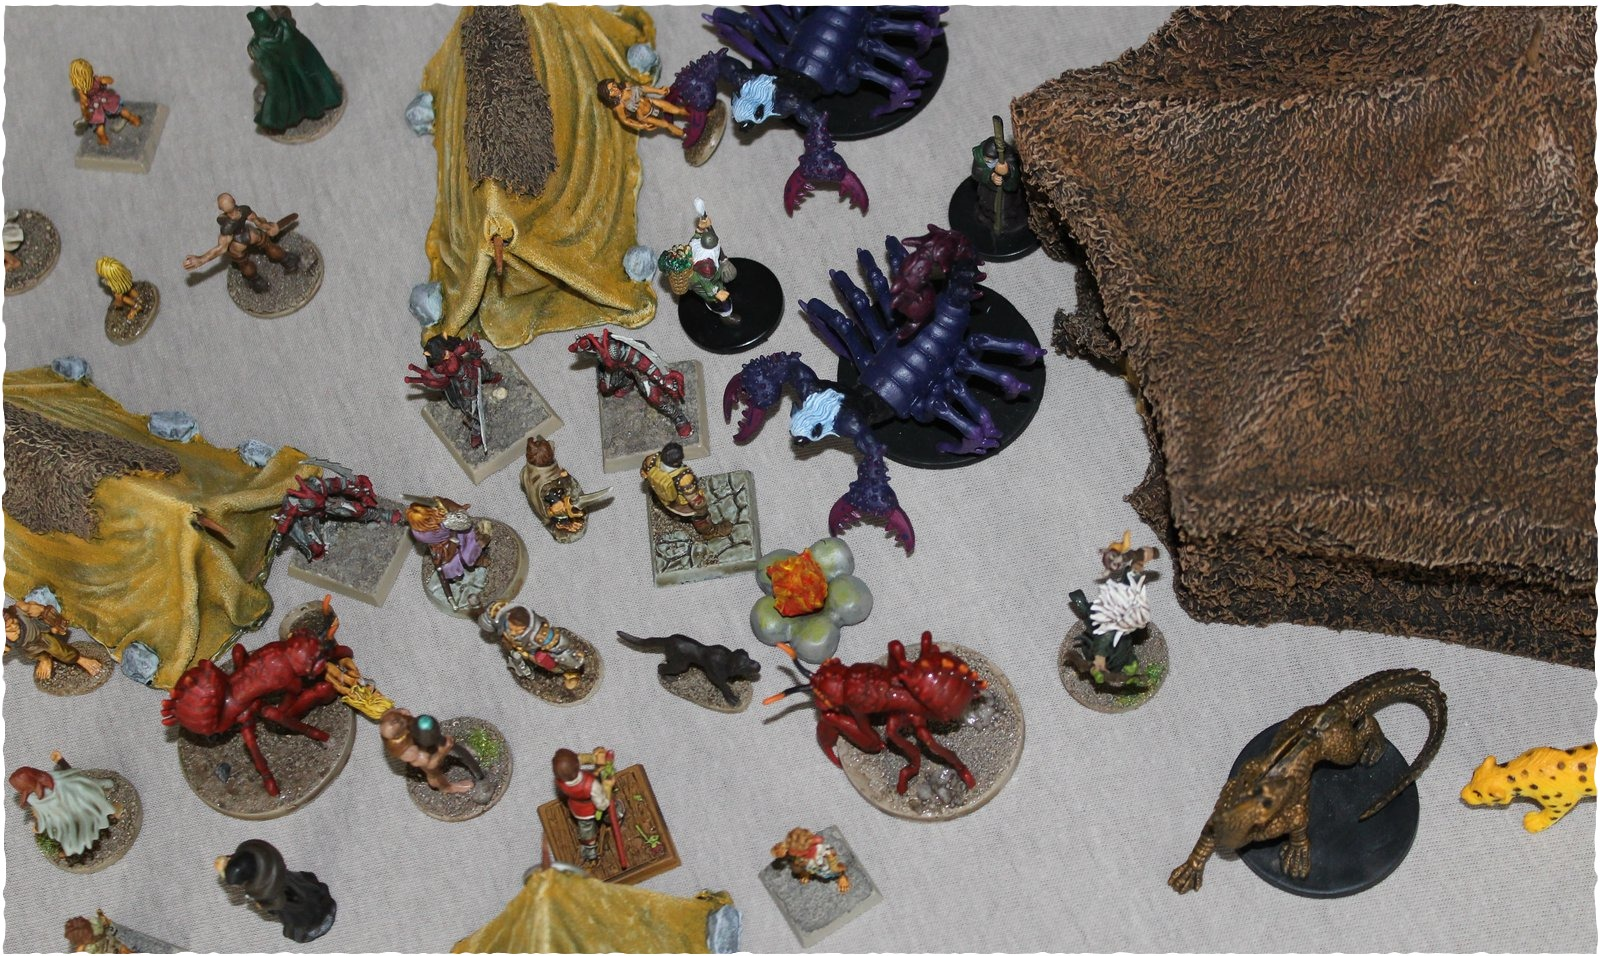
\includegraphics[width=0.4\textwidth]{images/Red-Mantis-assault-on-Shoanti-603326119_mod.jpg}
	\caption{Red Mantis assault on Shoanti}
	\label{fig:Red-Mantis-assault-on-Shoanti-603326119}
\end{figure}

With two fighters out of the game, it is time for some battlefield control: Sjo freezes the female assassin in place with {\itshape hold person} , but the archer resists a similar spell and a  {\itshape cacophonous call} from Quint. Next the bard makes the campfire explode in a bright flash, which blinds the male assassin, a scorpionman and the leopard, who is locked in combat with Wicked-Claws behind the main tent. Spyder suffers the same fate, but uses his instinct to continue his attacks anyway with surprising ease; naturally the blinded opponents try to do the same. Thousand Bones moves closer to \hyperref[fig:The-Cinderlander-from-Curse-of-the-Crimson-Throne-603327133]{ the source of the deadly bolts and recognizes the Cinderlander hiding behind a rocky outcropping. } The old medicine man finally manages to neutralize the danger by casting another  {\itshape hold person} on him, which finally succeeds. Meanwhile Puk takes out a first scorpion creature and deals heavy damage to the frozen female assassin. The wingless dragonne leaves the sight-robbed leopard groping in the dark and turns on the second giant mantis. Gushing blood from one of his wounds, unconscious Balian is in danger of bleeding out, so Sjo helps his friend with a  {\itshape cure critical wounds} . Quint and Thousand Bones provide further healing for the ranger, who tries to regain his feet. Despite his blindness Spyder manages to kill the female assassin next, who disappears in a puff of red smoke as well. Puk presses the final Red Mantis murderer, who takes down Sjo in turn. Fortunately Thousand Bones is close to lend assistance, one healer to another. Spyder continues his streak of good luck and finishes off the final assassin. Apparently the outdoor environment of the Cinderlands agree with the city dog. As the assassin pops away in red clouds, the giant mantis he summoned disappears as well. The only immediate threat left is the second scorpionman; the Cinderlander is still frozen in place and his blinded leopard pet is trying to find its way back to its master. Puk and Balian turn on the foul scorpion critter, drawing blood from many wounds, but still the creature persists and snaps and stings at the ranger with success as well. Fortunately Balian possesses enough fortitude to resist the poison. Puk is no big fan of the almost spiderlike way in which the giant scorpion creeps about, but with Balian providing flanking, he can duck between the creature's many legs and deliver the final blow. \\

\begin{figure}[h]
	\centering
	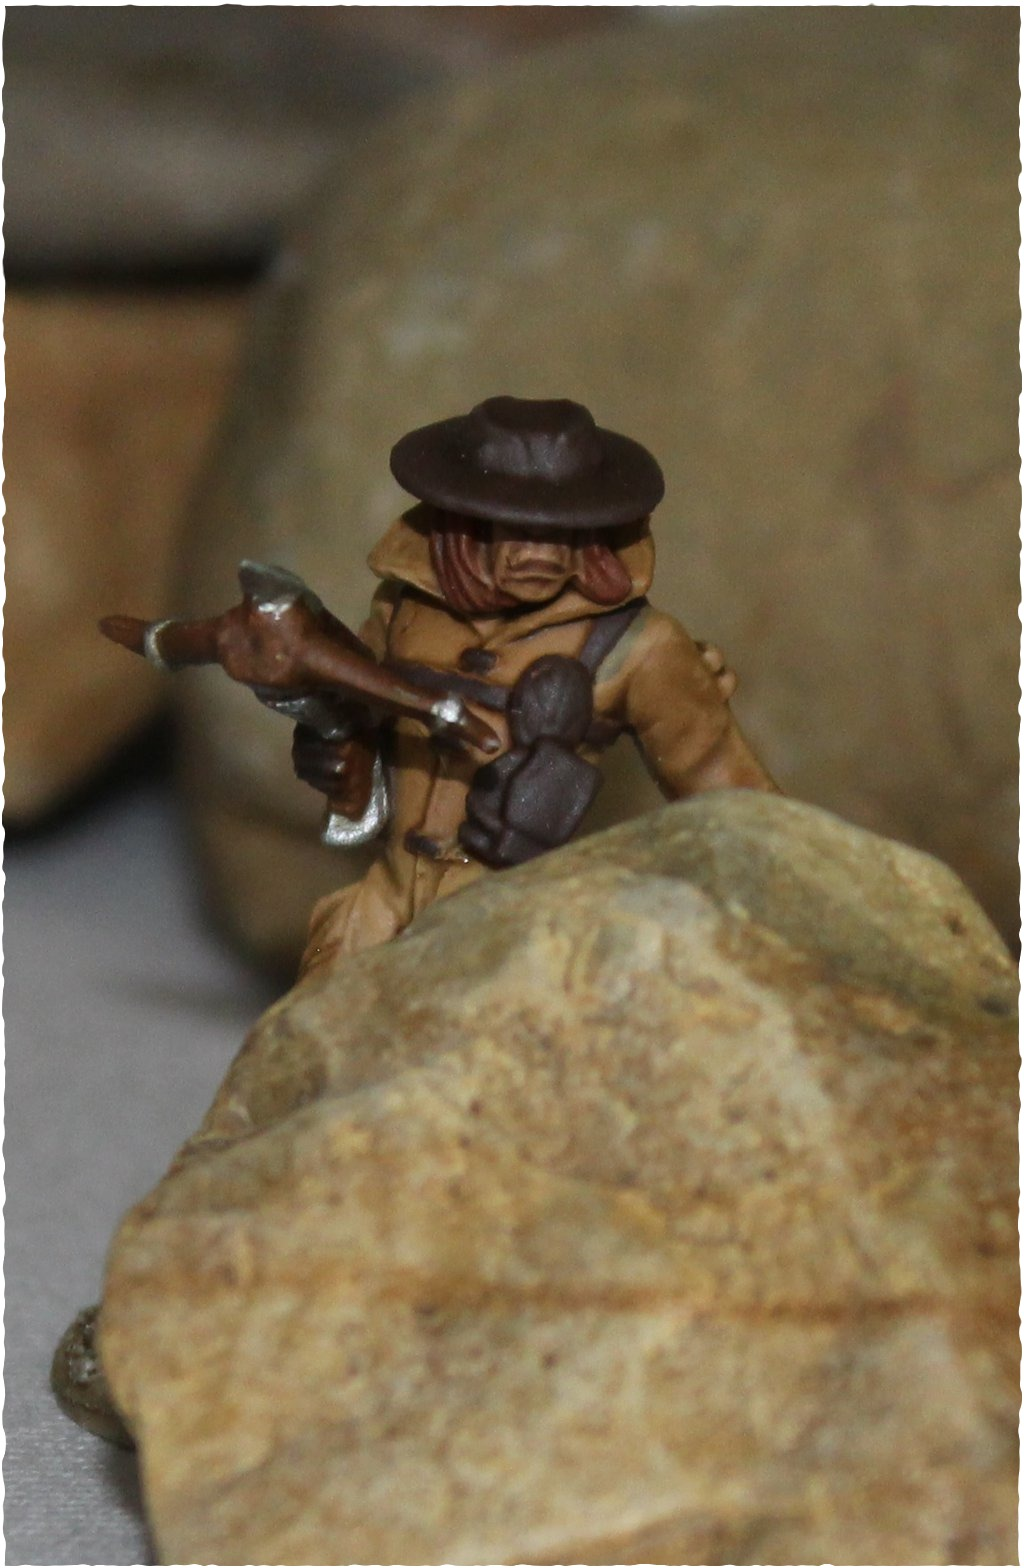
\includegraphics[width=0.4\textwidth]{images/The-Cinderlander-from-Curse-of-the-Crimson-Throne-603327133_mod.jpg}
	\caption{The Cinderlander from Curse of the Crimson Throne}
	\label{fig:The-Cinderlander-from-Curse-of-the-Crimson-Throne-603327133}
\end{figure}

Wasting no time, Balian charges over to the Cinderlander before the man manages to regain control of his movements. Wicked-Claws is close behind, chasing the leopard back to the archer, who finally breaks out of the {\itshape hold person} , but is laid low by another of Thousand Bones's spells. The old Shoanti  {\itshape commands} the Cinderlander to 'grovel', making the enemy fall prone in the dirt. \hyperref[fig:Death-of-the-Cinderlander-603327730]{ A storm of attacks from all sides ends his life. } By the time Sjo arrives it is already over, the Cinderlander is dead. So this deadly opponent was his biological father, was he? The healer cannot muster any pity for the man, but still sends him off with a short prayer to Pharasma. That is all the mercy this killer deserves. \\

\begin{figure}[h]
	\centering
	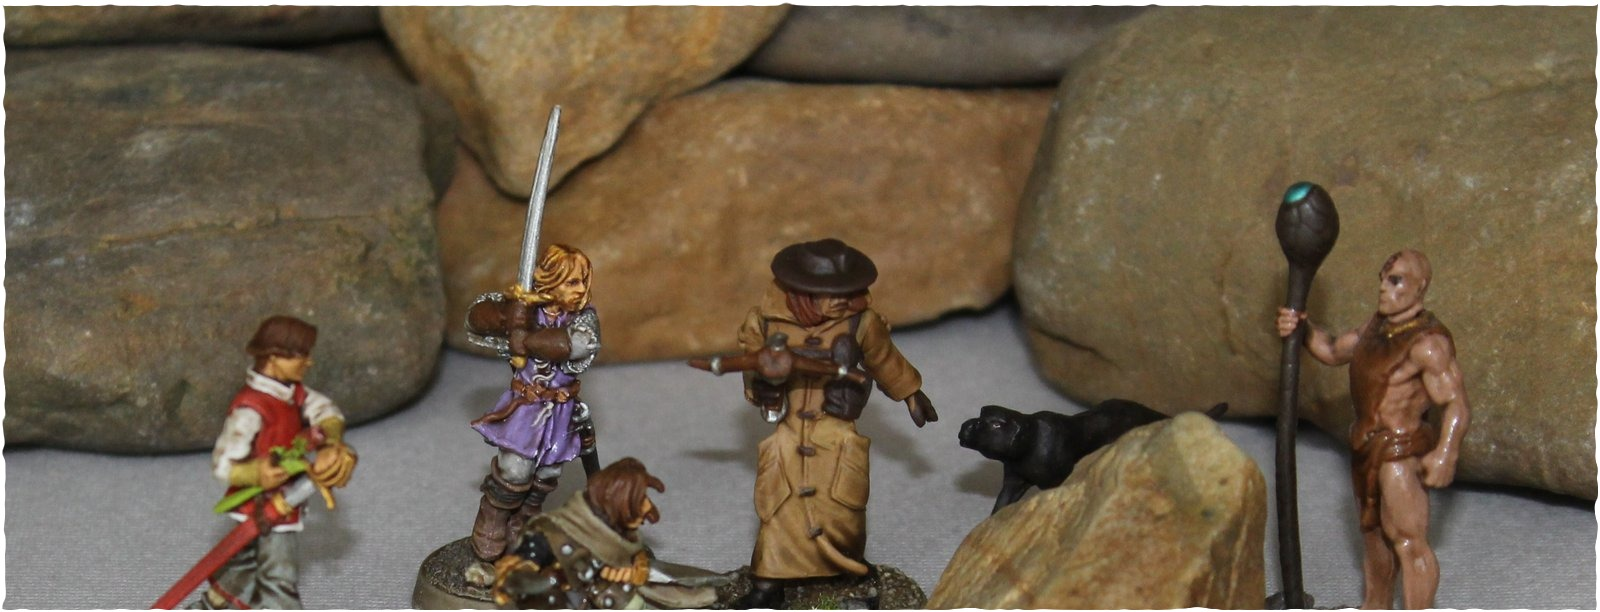
\includegraphics[width=0.4\textwidth]{images/Death-of-the-Cinderlander-603327730_mod.jpg}
	\caption{Death of the Cinderlander}
	\label{fig:Death-of-the-Cinderlander-603327730}
\end{figure}

Quint turns to Thousand Bones and says he is very sorry. This attack was aimed at his party, and it cost five innocent Shoanti bystanders their lives. Thousand Bones accepts his apology and says that at least one good thing came of it: the Cinderlander, who has been plaguing the Shoanti for almost two decades, is finally defeated. It is a sad day for the tribe, but a good day or all the clans in general. The victims will be honored as heroes and their names will live on in song and legend.\\

